\documentclass{jsarticle}
\usepackage[dvipdfmx]{graphicx}
\usepackage{listings,jlisting}
\usepackage{float}

\title{情報工学実験2 数理計画法 第二回}

\author{学生番号4617043 神保光洋}
\date{\today}
\begin{document}
\maketitle

\section{実験の要旨}
ハミング符号による符号化および符号プログラムの作成

\section{実験の目的}
誤り率を低くする。

\section{実験の原理}
$(n, k) = (7, 4)$ ハミング符号を用いる。$(7, 4)$ ハミング符号とは
代表的な誤り訂正符号の一つであり、単一誤りの訂正を可能とする。
符号化と呼ばれる操作によって4ビットの情報を7ビットの符号語に
変換し、送信する。

\section{実験方法}
今回自分はvisual studio2013 などという枯れた環境を使うこと
を嫌いUnix / Linuxのような再現可能かつ汎用性の高い環境で
実行を行うためあえてMTではなくrand()関数を使う
このあたりは評価されたい。
ちなみにTAには許可をいただいている。

\subsection{実験方法}
誤り訂正符号を用いる場合に置いて、$(7, 4)$ハミング符号に
よる符号化と符号を行うプログラムを作成する。
MTによって発生された乱数により$k = 4$ビットの
${0, 1}$の情報系列$w$を生成し、符号化により
$n - k = 7 - 4 = 3$ ビットの冗長ビットを算出し、
$n = 7$ビットの符号語$x$を生成する。また$n = 7$
ビットの符号語のうち誤りを付加させるビット位置
(1か所のみ)を指定できるように、受信系列$y$を
求める。復号によりどのビット位置
が誤っても訂正できることを確認する。
その雨に少なくとも複数の誤りパターンに
対し実行する

\section{実行環境}
Mojave 10.14.1
zsh 5.3 (x86\_64-apple-darwin18.0)
gcc 4.2.1

\section{結果}
プログラムの実行結果は以下のようになった
\begin{figure}[H]
  \centering
  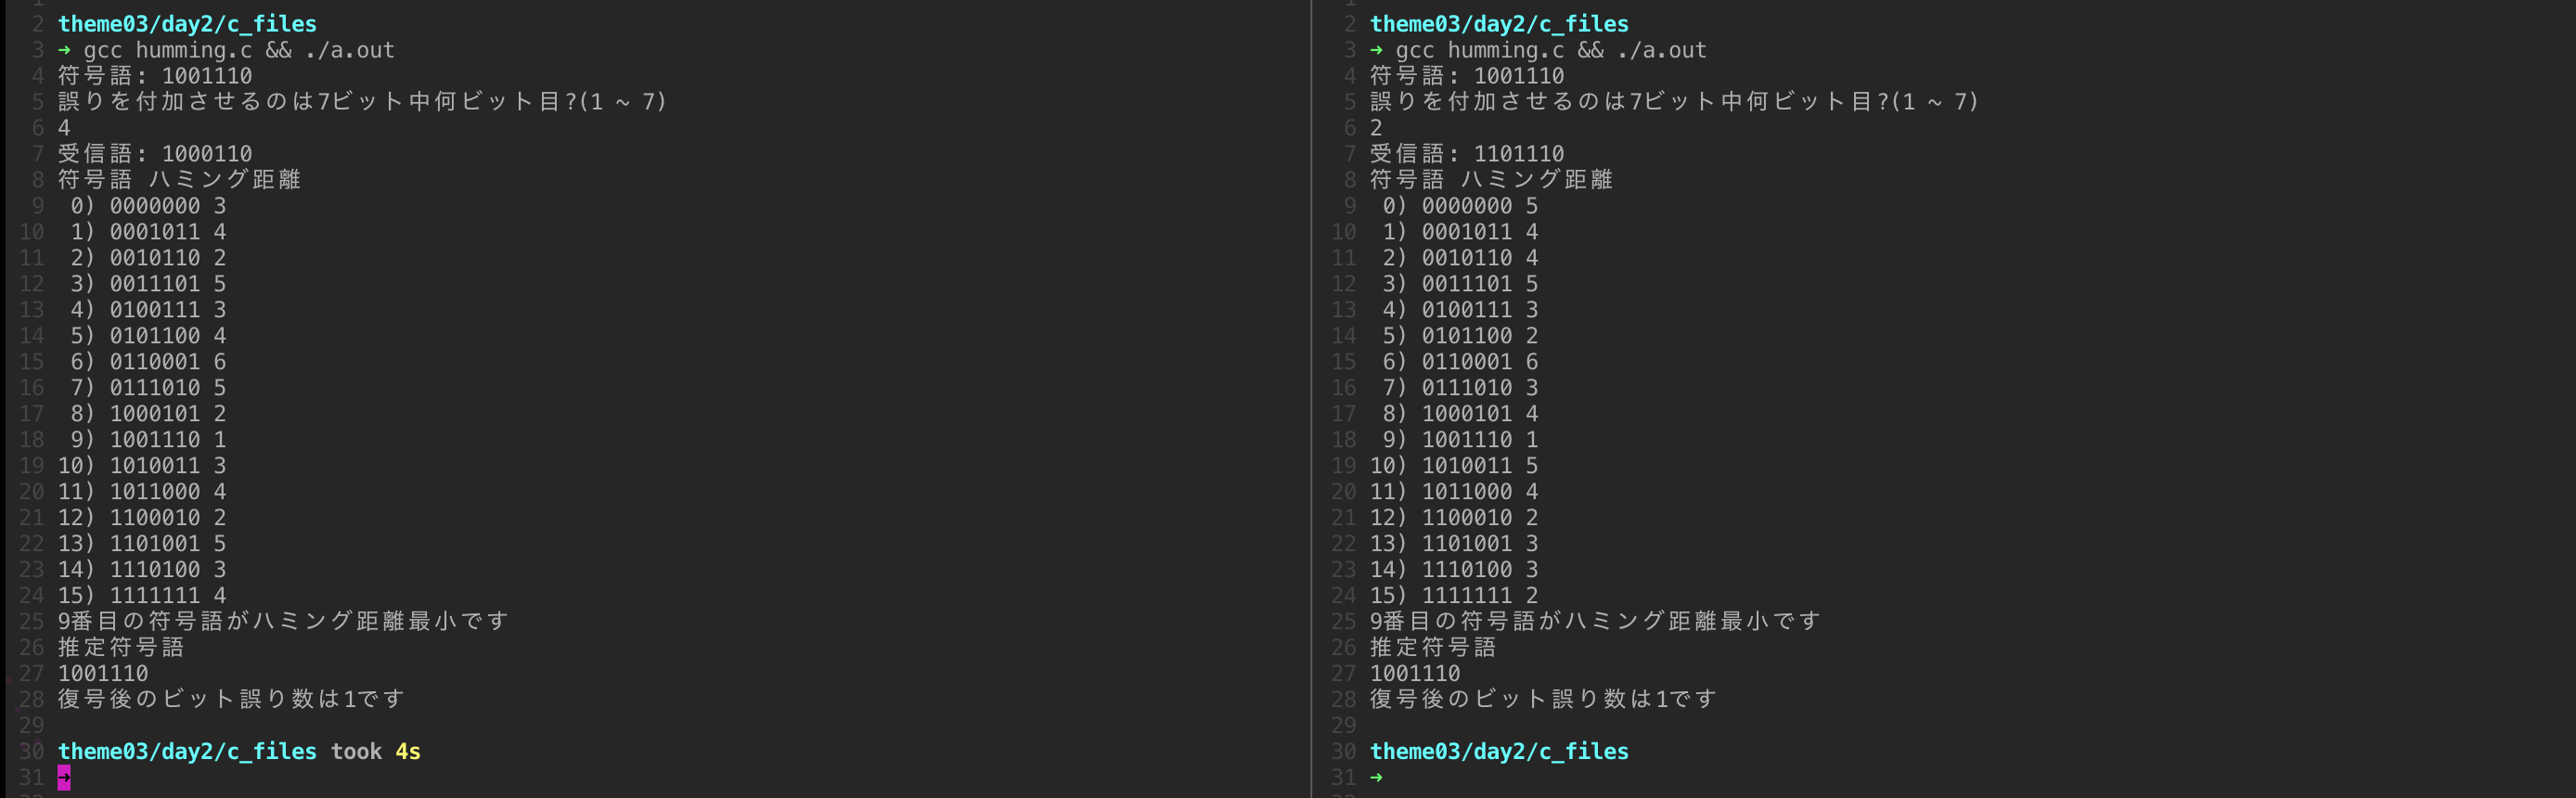
\includegraphics[width=12cm]{./result.png}
  \caption{最急降下法が生成した二次元配列}
\end{figure}

\section{検討事項}
\subsection{なぜハミング符号は1個誤りを訂正できるか}
の符号多項式を割り切ることができる $n − k$
次多項式で,かつ $x^n + 1$ の因数であるものを生成多項式
と言う。今回のハミング符号はこれで生成される
多項式を割り、そのあまりを求める。
これにより符号を分割することができる。 
誤りが1つの場合16個の多項式表現を一意に表すことが
できる、これはハミング符号1個誤りを一意に表すことを
意味する。

\subsection{2個以上の誤りが発生するとどうなるか。2個、3個、...とするとどうなるか。}
上にも触れた通り誤りが1つの場合16個の多項式表現を一意に
表すことができるが2つ以上であると一意に定めることはできなくなる。
しかしどれかどれであると言ったような推定は誤りが少なければ
できる2個、3個となるほどに受信語$y$とのハミング距離は増え誤りの推定値は増える

\subsection{まとめ}
ハミング距離は自然言語処理などで使われることは
知っていたが情報通信でも使われていることを理解した。

また誤りが多いと誤り訂正符号は推定できなくなることを実験を通し学んだ。

\section{参考文献}
\begin{thebibliography}{9}
  \bibitem{key1} 山本和彦 プログラミングHaskell・オーム社
  \bibitem{key2} 高橋麻奈 やさしいC言語(第5版)・SBクリエイティブ
\end{thebibliography}

\section{付録}
実験で使用したプログラムは以下のようになる。
\lstinputlisting[caption = humming.c ,label = program1]{./humming.c}

\end{document}
